% !TEX root = ../thesis.tex
%
\chapter{Einleitung}
\label{sec:intro}
Wikipedia ist die bekannteste freie Wissenssammlung im Internet.
Bei fast 50 Millionen Artikeln in 278 Sprachen\footnote{https://stats.wikimedia.org/DE/TablesArticlesTotal.htm} Anfang 2019 sind Informationen zu einer Vielfalt an Themen verfügbar.
Sogar YouTube und Facebook greifen auf Wikipedia zurück, um zusätzliche Informationen zu kontroversen Themen zu präsentieren\cite{youtube-facebook-wp}.

Die Darstellung der Informationen in natürlicher Sprache als Textartikel ist für Menschen praktisch.
Die Extraktion von Fakten für die maschinelle Verarbeitung aus diesen Textartikel ist jedoch schwierig\cite{oie-errors}\cite{extract-rel-ibm}.
Das Problem wird durch die unterschiedlichen Sprachversionen noch verstärkt, denn die beschriebenen Fakten können sich je nach Sprache unterscheiden.
Um diesem Problem zu entgegnen wurde 2012 das Wikidata Projekt gegründet, mit dem Ziel, die Informationen aus Wikipedia in atomare Aussagen zerlegt strukturiert zu verwalten\cite{wikidata}.

Als Datensatz ist Wikidata für viele Anwendungen interessant, da er detaillierte Fakten zu einem breiten Themengebiet liefert.
Je nach Art der Bestimmung kann beispielsweise entweder der Mount Everest oder Chimborazo als höchster Punkt der Erde gesehen werden.
Das Datenmodell von Wikidata kann beide Sichtweisen abbilden, wie \cref{fig:sample-statement} zeigt.
Wikidata ist wie Wikipedia ein Community-Projekt, dass von jedem frei bearbeitet werden kann.
Um die Herkunft einer Information zu belegen, kann jeder Fakt mit Referenzen versehen werden.

Aus dieser große Datenmenge ergeben sich auch Herausforderungen.
Im September 2019 hat die Größe des vollständigen Exports der Daten als GZip\footnote{\url{http://www.gzip.org/}}-komprimiertes JSON\footnote{\url{https://www.json.org}} (JavaScript Object Notation) 60 GB überschritten\footnote{\url{https://web.archive.org/web/20190930113616/https://dumps.wikimedia.org/wikidatawiki/entities/}}.
Für viele Anwendungen sind aber nicht alle Daten relevant.
Ziel dieser Arbeit ist deswegen die Entwicklung eines Systems zum einfachen Abruf einer Teilmenge dieser Daten.

\begin{figure}
  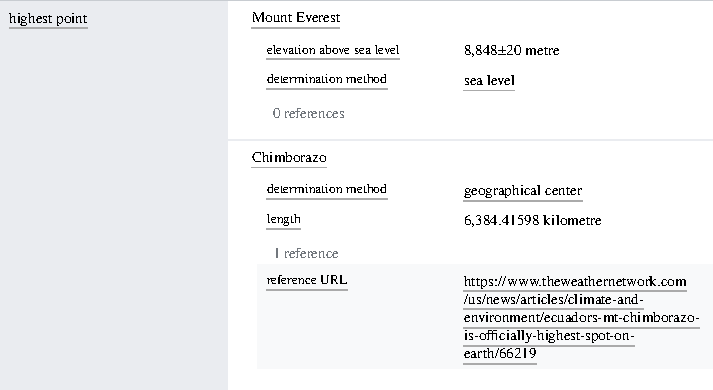
\includegraphics[width=\linewidth]{pics/example-statement}
  \caption{Zwei Statements des Items ``Erde'' für die Property ``höchster Punkt''}
  \label{fig:sample-statement}
\end{figure} 

Der Wikidata Query Service\footnote{\url{https://query.wikidata.org/}} ist für diese Aufgabe nicht ausreichend.
Da die Laufzeit von Abfragen auf eine Minute limitiert ist, eignet sich dieser nur für kleinere Datenmengen.
Das dieses Limit nicht nur ein theoretisches Problem ist, zeigt eine Arbeit zur Verwendung von Referenzen in Wikidata\cite{wd-wk-common-references}.
Die Autoren mussten die Abfrage nach allen Referenzen von einem Mitarbeiter von Wikimedia Deutschland ausführen lassen, da sie nicht innherhalb des Limits terminiert.

Das in dieser Arbeit vorgestellte System füllt die Nische zwischen dem vollständigen Export und dem Wikidata Query Service.
Durch die Angabe von Filtern wird eine Teilmenge der Daten definiert.
Aus den Daten, die diese Filter erfüllen, wird dann ein Dump generiert.
Über eine Integration mit Zenodo\footnote{\url{https://zenodo.org/}} können die generierten Dumps direkt archiviert werden.
Zenodo generiert einen Digital Object Identifier (DOI), sodass die Dumps danach einfach in wissenschaftlichen Veröffentlichungen zitiert werden können.

\section{Struktur der Arbeit}
Im zweiten Kapitel wird zunächst notwendiges Hintergrundwissen zum Aufbau von Wikidata und den verwendeten Technologien vermittelt.
Danach werden in \cref{chap:requirements} die Anforderung an das System detaillierter beschrieben und verwandete Arbeiten verglichen.
In \cref{chap:design} wird dann das Design der System erarbeitet, dessen Implementierung in \cref{chap:implementation} vorgestellt wird.
In der folgenden Evaluation in \cref{chap:evaluation} wird die Implementierung auf Erreichen der Anforderung geprüft und auch ein Vergleich mit den existierenden Wikidata-Dumps vorgenommen.
Im letzten Kapitel \cref{chap:conclusion} wird schließlich ein Ausblick auf mögliche Verbesserungen gegeben und eine Zusammenfassung des Ergebnis präsentiert.

Dabei werden die folgenden Beiträge geleistet:
\begin{itemize}
  \item Analyse verschiedener Systemdesigns zur Generierung angepasster Wikidata-Dumps
  \item Entwurf einer Spezifikation für Filterkriterien
  \item Implementierung des vorgestellten Designs mit Wikidata-Toolkit
  \item Evaluation der Vollständigkeit und Korrektheit des RDF-Exports von Wikidata-Toolkit
\end{itemize}